\documentclass[tikz,border=10pt]{standalone}
% Shared style for all project diagrams
\usepackage{amsmath,amssymb}
\usetikzlibrary{positioning,arrows.meta,calc,fit,decorations.pathreplacing}
\renewcommand{\familydefault}{\sfdefault}
\definecolor{accent}{RGB}{42,120,214}
\definecolor{lblue}{RGB}{234,242,252}
\definecolor{card}{RGB}{247,247,245}
\definecolor{ink}{RGB}{17,17,17}
\definecolor{gray52}{RGB}{82,81,78}
\definecolor{dblue}{RGB}{13,54,107}
\tikzset{
  box/.style={draw=accent, thick, rounded corners=3pt, fill=lblue, align=center,
              minimum height=1.05cm, inner sep=6pt, text=ink},
  plain/.style={draw=gray52!60, thick, rounded corners=3pt, fill=card, align=center,
              minimum height=1.05cm, inner sep=6pt, text=ink},
  ghost/.style={align=center, text=gray52, font=\footnotesize},
  arr/.style={-{Stealth[length=2.6mm]}, very thick, draw=accent},
  garr/.style={-{Stealth[length=2.6mm]}, thick, draw=gray52},
  lbl/.style={font=\footnotesize, text=gray52, align=center},
}

\begin{document}
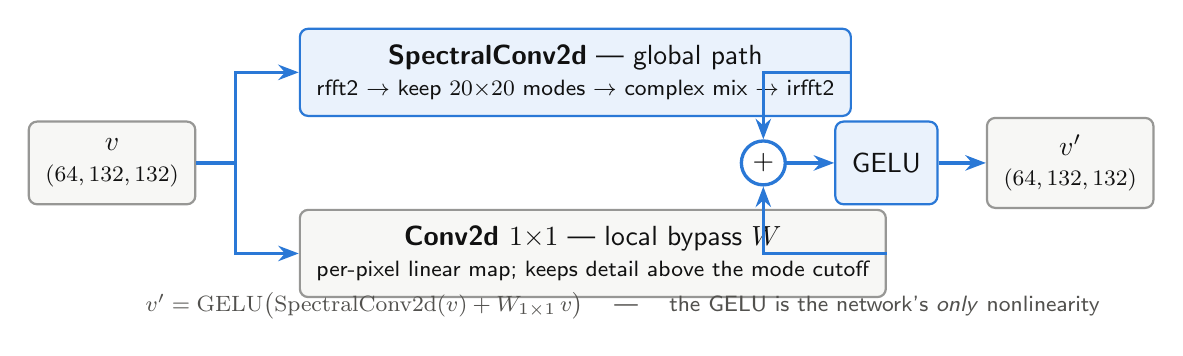
\begin{tikzpicture}[node distance=0.7cm and 1.0cm]
  \node[plain] (vin) {$v$\\[-1pt] {\footnotesize $(64,132,132)$}};

  \node[box, right=1.3cm of vin, yshift=1.15cm, minimum width=5.6cm] (spec)
    {\textbf{SpectralConv2d} --- global path\\[-1pt]
     {\footnotesize rfft2 $\to$ keep $20{\times}20$ modes $\to$ complex mix $\to$ irfft2}};

  \node[box, right=1.3cm of vin, yshift=-1.15cm, minimum width=5.6cm, fill=card, draw=gray52!60] (loc)
    {\textbf{Conv2d $1{\times}1$} --- local bypass $W$\\[-1pt]
     {\footnotesize per-pixel linear map; keeps detail above the mode cutoff}};

  \node[circle, draw=accent, very thick, fill=white, inner sep=2pt, right=6.9cm of vin] (add) {$+$};
  \node[box, right=0.6cm of add] (act) {GELU};
  \node[plain, right=0.6cm of act] (vout) {$v'$\\[-1pt] {\footnotesize $(64,132,132)$}};

  \draw[arr] (vin.east) -- ++(0.5,0) |- (spec.west);
  \draw[arr] (vin.east) -- ++(0.5,0) |- (loc.west);
  \draw[arr] (spec.east) -| (add.north);
  \draw[arr] (loc.east)  -| (add.south);
  \draw[arr] (add) -- (act);
  \draw[arr] (act) -- (vout);

  \node[lbl, below=2.1cm of spec, xshift=0.6cm]
    {$v' = \mathrm{GELU}\bigl(\mathrm{SpectralConv2d}(v) + W_{1\times1}\,v\bigr)$
     \quad --- \quad the GELU is the network's \emph{only} nonlinearity};
\end{tikzpicture}
\end{document}
